\documentclass[IEEEtran,letterpaper,10pt,notitlepage,draftclsnofoot,onecolumn]{article}

\usepackage{nopageno}
\usepackage{alltt}
\usepackage{float}
\usepackage{color}
\usepackage{balance}
\usepackage{enumitem}
\usepackage{pstricks, pst-node}
\usepackage{geometry}
\geometry{textheight=9.5in, textwidth=7in}
\newcommand{\cred}[1]{{\color{red}#1}}
\newcommand{\cblue}[1]{{\color{blue}#1}}
\usepackage{hyperref}
\usepackage{textcomp}
\usepackage{listings}
\usepackage{titling}
\usepackage{graphicx}
\usepackage{url}
\usepackage{setspace}
\usepackage{tabular}
\usepackage{fancyhdr}
\pagestyle{fancy}
\fancyfoot[C]{REQDELTA--\thepage}

\begin{document}
\begin{sloppypar}
\section{Changes to the requirements}
\begin{tabular}{|p{.1cm}|l|p{2cm}| p{5cm} |} 
 \hline
 1 & Use Kinetic Kame as our ROS distribution & Used Indigo Igloo instead & The older version of ROS was more commonly used in other code samples, so the team used it instead for compatibility\\
 \hline
 2 & Submit patches for vulnerabilites upstream & Didn't create any patches & All the vulnerabilities we found were based in how ROS was designed, not a code exploit or bug. So there really was not anything to patch.\\
 \hline
\end{tabular}
\\ \\ 
\end{sloppypar}
\begin{figure}[ht!]
\centering
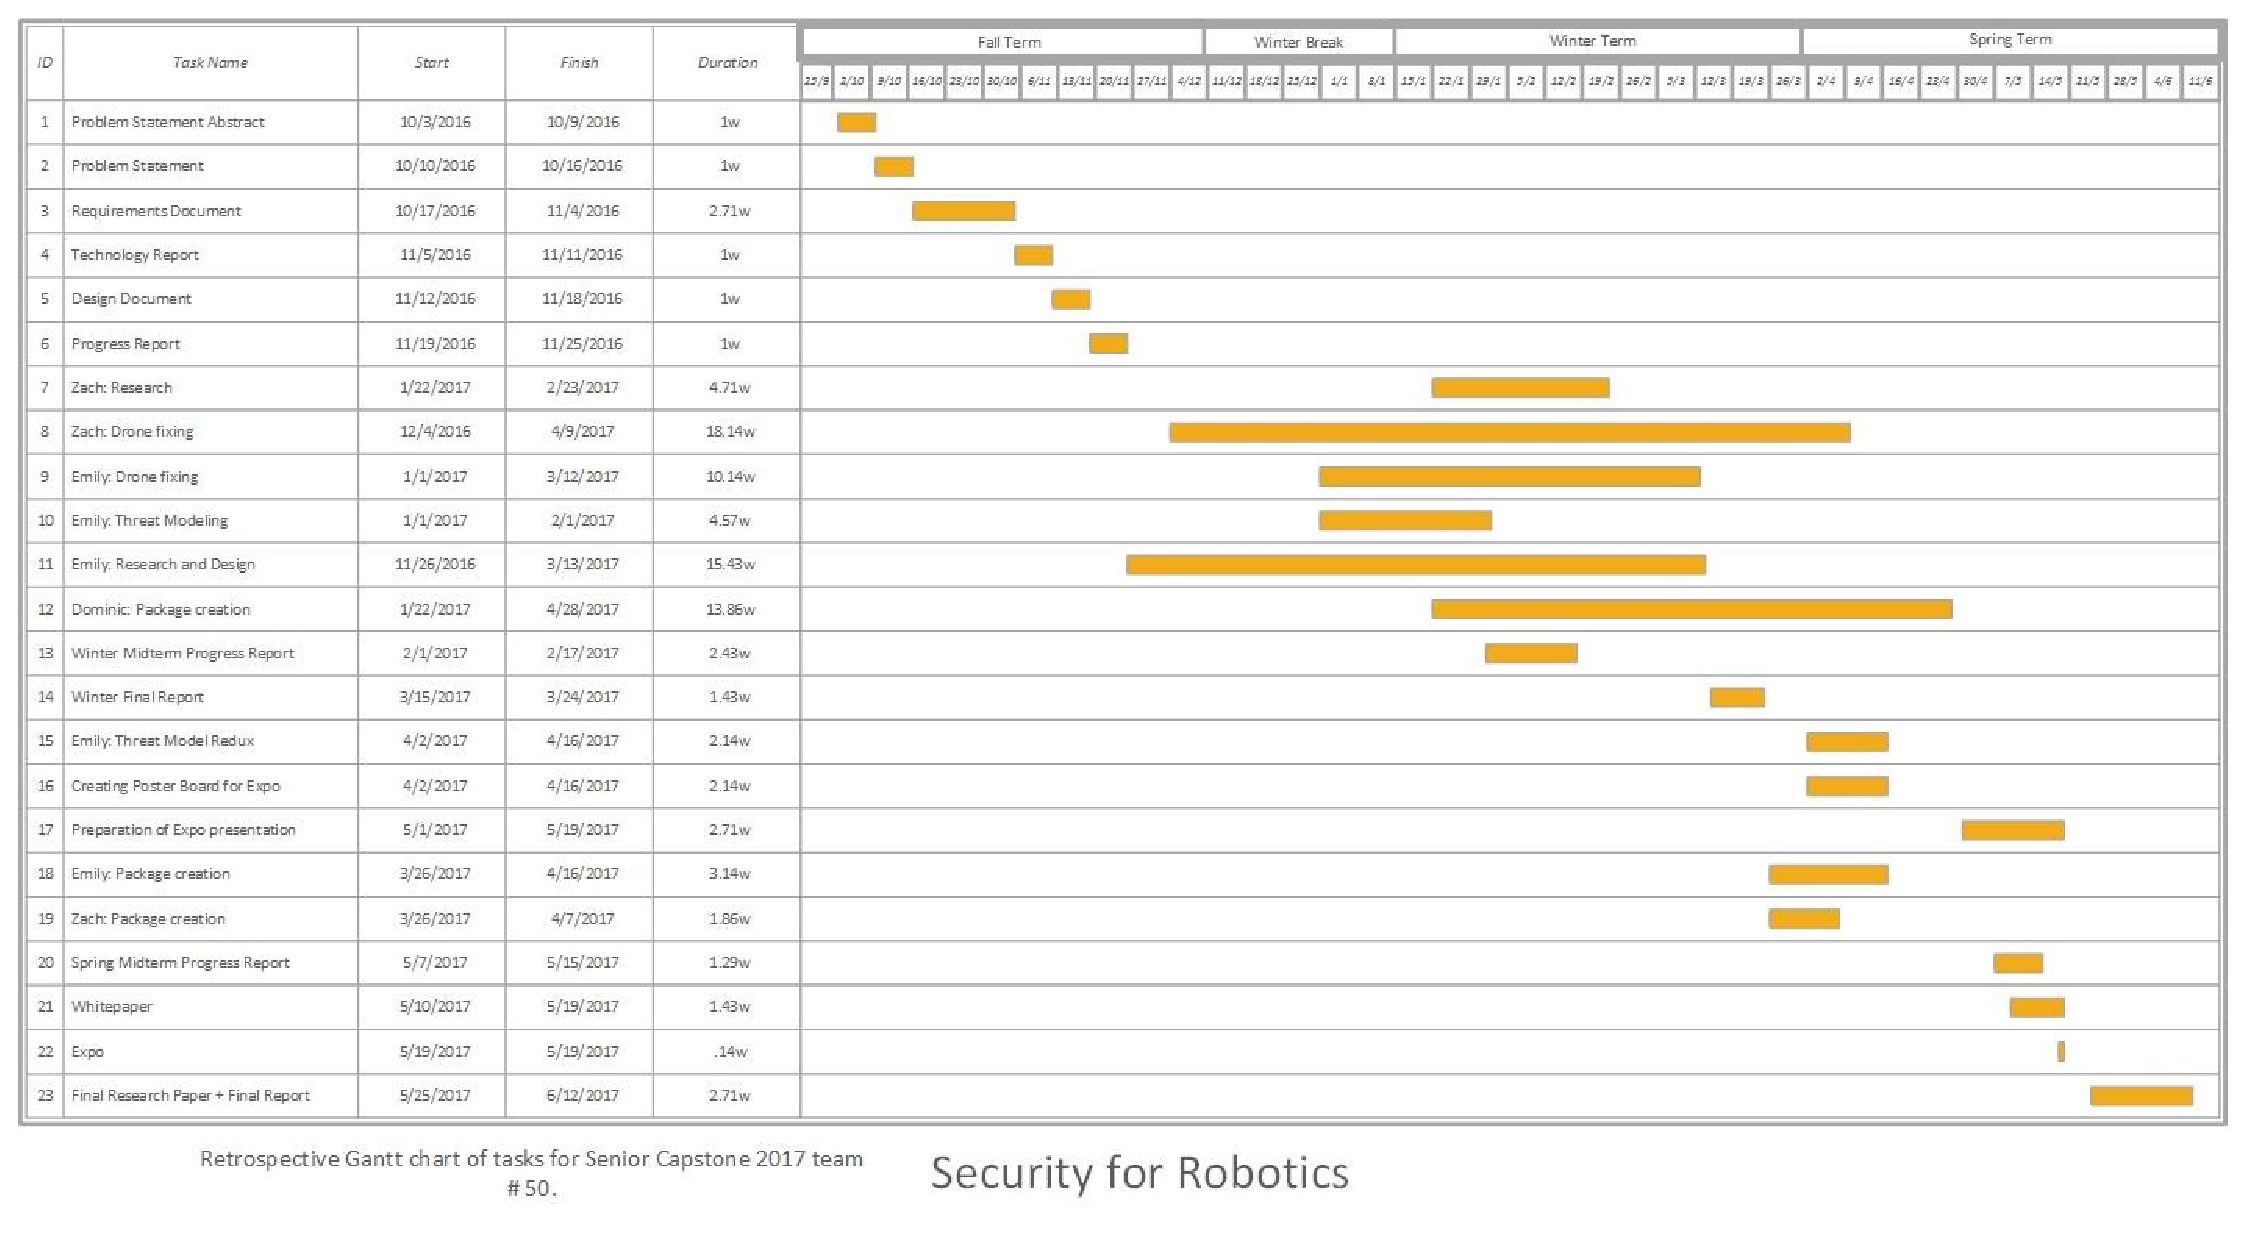
\includegraphics[width=170mm]{finalgannt.eps}
\end{figure}
%
%The only explicit change we had to our requirements was that our team used 
%ROS Indigo Igloo over Kinetic Kame, as a large part of the existing ROS codebase
%was created during Indigo and Kame had some compatibility issues with some 
%Indigo-based code. There was also the understanding that we would not be 
%producing patches to patch any vulnerabilities we found, as all of them
%stem from underlying design choices in ROS itself rather than programming
%errors. This makes everything more or less unpatchable, as it would require
%design changes to ROS itself that are simply not in consideration by the 
%ROS development team. In turn, since our team produced no patches, we did 
%not send them to the SROS project for consideration either.
\end{document}
